\documentclass[12pt]{article}
\usepackage[margin=1in]{geometry}                % See geometry.pdf to learn the layout options. There are lots.
\geometry{letterpaper}                   % ... or a4paper or a5paper or ... 
%\geometry{landscape}                % Activate for for rotated page geometry
\usepackage[parfill]{parskip}    % Activate to begin paragraphs with an empty line rather than an indent

%%%%%%%%%%%%%%%%%%%%
\newcommand{\hide}[1]{}



\usepackage{natbib}
\usepackage{xcolor}
\usepackage{url}
\usepackage{hyperref}
\usepackage{mathtools}
\usepackage[utf8]{inputenc}
\usepackage{float}
\usepackage{listings}
\usepackage{xcolor}


\hide{
\usepackage{amscd}
\usepackage{amsfonts}
\usepackage{amsmath}
\usepackage{amssymb}
\usepackage{amsthm}
\usepackage{cases}		 
\usepackage{cutwin}
\usepackage{enumerate}
\usepackage{enumitem}
\usepackage{epstopdf}
\usepackage{graphicx}
\usepackage{ifthen}
\usepackage{lipsum}
\usepackage{mathrsfs}	
\usepackage{multimedia}
\usepackage{wrapfig}
}
\bibliographystyle{humanbio}


\usepackage[utf8]{inputenc}

\newcommand{\itemlist}[1]{\begin{itemize}#1\end{itemize}}
\newcommand{\enumlist}[1]{\begin{enumerate}#1\end{enumerate}}
\newcommand{\desclist}[1]{\begin{description}#1\end{description}}
\newcommand\tab[1][0.5cm]{\hspace*{#1}}

\newcommand{\Answer}[1]{\begin{quote}{\color{blue}#1}\end{quote}}
\newcommand{\AND}{\wedge}
\newcommand{\OR}{\vee}
\newcommand{\ra}{\rightarrow}
\newcommand{\lra}{\leftrightarrow}

\title {{\bf ECE 471 Lab 3} \\
\large{MD5 Collision Attack Lab}}

\author{Mitchell Dzurick}
\date{3/9/2020}
\begin{document}

\maketitle
\textbf{Github with all documentation - \url{https://www.github.com/mitchdz/ECE471}}
\tableofcontents 

\clearpage


Secret Key Encryption Lab

Copyright © 2018 Wenliang Du, Syracuse University. The development of this document was partially funded by the National
Science Foundation under Award No. 1303306 and 1718086. This work is licensed under a Creative Commons
Attribution-NonCommercial- ShareAlike 4.0 International License. A human-readable summary of (and not a substitute for)
the license is the following: You are free to copy and redistribute the material in any medium or format. You must give
appropriate credit. If you remix, transform, or build upon the material, you must distribute your contributions under the
same license as the original. You may not use the material for commercial purposes.

\section{Overview}

A secure one-way hash function needs to satisfy two properties: the one-way property and the collision-
resistance property. The one-way property ensures that given a hash value h, it is computationally infeasible
to find an input M , such that hash(M ) = h. The collision-resistance property ensures that it is compu-
tationally infeasible to find two different inputs M 1 and M 2 , such that hash(M 1 ) = hash(M 2 ).
Several widely-used one-way hash functions have trouble maintaining the collision-resistance prop-
erty. At the rump session of CRYPTO 2004, Xiaoyun Wang and co-authors demonstrated a collision attack
against MD5 [1]. In February 2017, CWI Amsterdam and Google Research announced the SHAttered at-
tack, which breaks the collision-resistance property of SHA-1 [3]. While many students do not have trouble
understanding the importance of the one-way property, they cannot easily grasp why the collision-resistance
property is necessary, and what impact these attacks can cause.
The learning objective of this lab is for students to really understand the impact of collision attacks, and
see in first hand what damages can be caused if a widely-used one-way hash function’s collision-resistance
property is broken. To achieve this goal, students need to launch actual collision attacks against the MD5
hash function. Using the attacks, students should be able to create two different programs that share the
same MD5 hash but have completely different behaviors. This lab covers a number of topics described in
the following:


    \begin{itemize}
        \item One-way hash function
        \item The collision-resistance property
        \item Collision attacks
        \item MD5
    \end{itemize}

\textbf{Lab Environment}. This lab has been tested on our pre-built Ubuntu 12.04 VM and Ubuntu 16.04 VM, both of which
can be downloaded from the SEED website.

\clearpage
\section{Lab Tasks}
\section{Task 1: Generating Two Different Files with the Same MD5 Hash}
In this task, we will generate two different files with the same MD5 hash values. The beginning parts of these
two files need to be the same, i.e., they share the same prefix. We can achieve this using the md5collgen
program, which allows us to provide a prefix file with any arbitrary content. The way how the program works
is illustrated in Figure 1. The following command generates two output files, out1.bin and out2.bin,
for a given a prefix file \emph{prefix.txt}:

\begin{verbatim}
$ md5collgen -p prefix.txt -o out1.bin out2.bin
\end{verbatim}

\begin{figure}[H]
	\begin{center}
		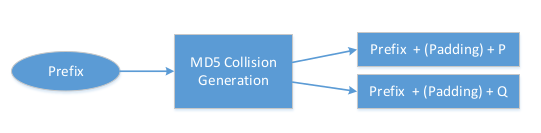
\includegraphics[scale=0.6]{pics/i1.png}
	\end{center}{}
	\caption{Running the key generation program without srand multiple times}
	\label{fig:i1}
\end{figure}

We can check whether the output files are distinct or not using the diff command. We can also use the
md5sum command to check the MD5 hash of each output file. See the following commands.
\begin{verbatim}
$ diff out1.bin out2.bin
$ md5sum out1.bin
$ md5sum out2.bin
\end{verbatim}

\tab Since out1.bin and out2.bin are binary, we cannot view them using a text-viewer program, such
as cat or more; we need to use a binary editor to view (and edit) them. We have already installed a hex
editor software called bless in our VM. Please use such an editor to view these two output files, and
describe your observations. In addition, you should answer the following questions:
\begin{itemize}
	\item Question 1. If the length of your prefix file is not multiple of 64, what is going to happen?
	\item Question 2. Create a prefix file with exactly 64 bytes, and run the collision tool again, and see what happens.
	\item Question 3. Are the data (128 bytes) generated by md5collgen completely different for the two
output files? Please identify all the bytes that are different.	
\end{itemize}



\subsection{Task 1 Solution}

Initial observations are required in the md5collgen program. To do this, let's execute the program.

\begin{figure}[H]
	\begin{center}
		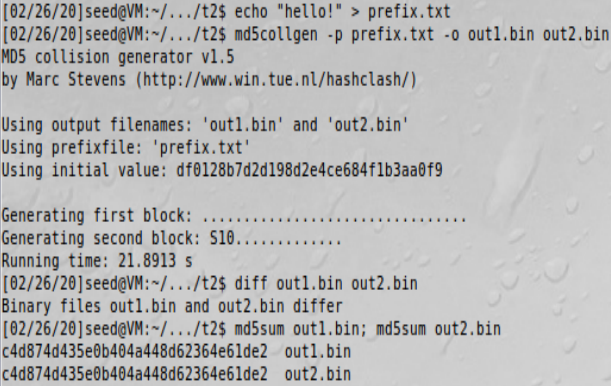
\includegraphics[scale=0.65]{pics/t1p00.png}
	\end{center}{}
	\caption{investigating md5collgen program}
	\label{fig:t1p00}
\end{figure}

As Figure~\ref{fig:t1p00} shows, a file with the contents "hello!" being thrown into md5collgen. The output is two files, named "out1.bin" and "out2.bin". These hash of these files are then produced using the commands md5sum. It can be seen that the files are different through the `diff` command, but their md5sum hash is the same.

\subsubsection{Task 1 Question 1 Solution}
the prefix was padded with zero bytes until the size is a multiple of 64.
\begin{figure}[H]
	\begin{center}
		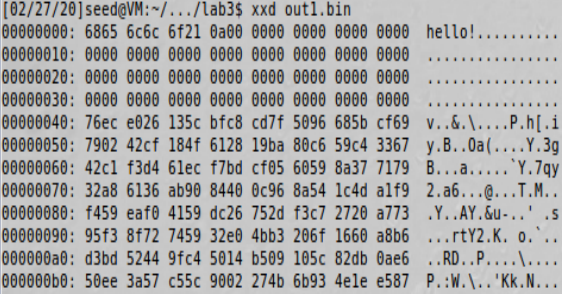
\includegraphics[scale=0.65]{pics/t1p3.png}
	\end{center}{}
	\caption{file not of 64 bytes being ran through md5collgen}
	\label{fig:t1p3}
\end{figure}

Figure~\ref{fig:t1p3} shows the results from Figure~\ref{fig:t1p00}. out1.bin is shown to be padded with 0's until 64 bytes, then seemingly random data is appended.

\subsubsection{Task 1 Question 2 Solution}
With 64-byte prefix, no bytes are needed for padding. The prefix then has extra data added on for the collision. Figure~\ref{fig:t1p1} shows these results as there is no extra 0 bytes added, but rather just extra data to aid in the collision.


\subsubsection{Task 1 Question 3 Solution}
A file named prefix.txt is created with contents "Hello! I am a test sentence that is trying to fill up 64 bytes." this file is then ran through the md5collgen.

\begin{figure}[H]
	\begin{center}
		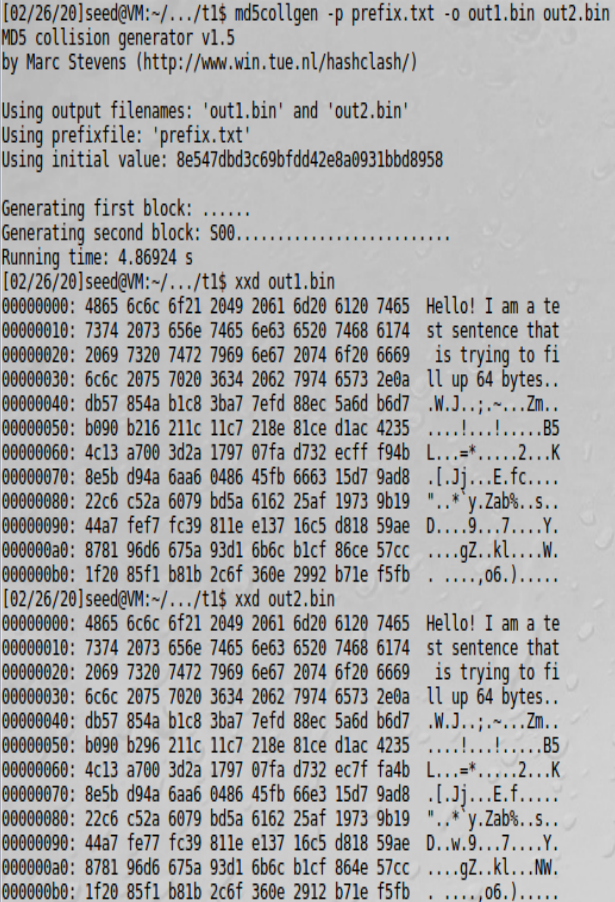
\includegraphics[scale=0.65]{pics/t1p1.png}
	\end{center}{}
	\caption{64 bytes of prefix being put into the md5collgen}
	\label{fig:t1p1}
\end{figure}

Figure~\ref{fig:t1p1} shows that the files don't completely differ, but they do differ in certain areas. It's actually apparent that only 8 bytes are different out of the 192 bytes that are output. The bytes that changed only changed a little bit as well. They only differ in one bit.


\subsection{Task 2: Understanding MD5's Property}
\subsubsection{Task 2: Solution}




In order to finish this task, some setup is required. To generate all of the files, the commands below are executed.
\begin{verbatim}
echo "hello!" > prefix.txt
md5collgen -p prefix.txt -o out1.bin out2.bin
echo "T" > T
cat out1.bin T > T1
cat out2.bin T > T2
\end{verbatim}

These commands will generate the following files: T, out1.bin, out2.bin, T1, T2. T is a file that contains the hex value "0x540a" because of the \emph{echo "T" > T} command. out1.bin and out2.bin are the files generated by md5collgen which their hash values match as shown in Figure~\ref{fig:t2p1}.

\begin{figure}[H]
	\begin{center}
		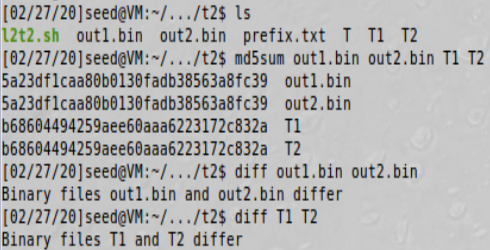
\includegraphics[scale=0.65]{pics/t2p1.png}
	\end{center}{}
	\caption{matching md5sum values}
	\label{fig:t2p1}
\end{figure}

Figure~\ref{fig:t2p1} shows the results of running all of the aforementioned commands. It can be seen that the md5 value of out1.bin and out2.bin match, and the md5sum value of T1 and T2 also match. Below that, the command `diff` is used to show that the binary value of every file is different, yet they produce the same hash.


\begin{figure}[H]
	\begin{center}
		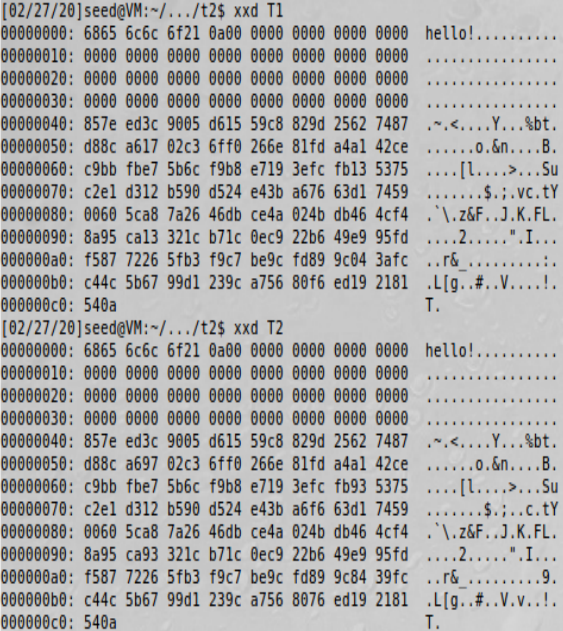
\includegraphics[scale=0.65]{pics/t2p2.png}
	\end{center}{}
	\caption{hex values of output}
	\label{fig:t2p2}
\end{figure}
 
Figure~\ref{fig:t2p2} also shows the hex values of T1 and T2 which shows that 0x540a is appended to each file.

\subsection{Task 3: Generating Two Executable Files with the Same MD5 Hash}
\subsubsection{Task 3: Solution}

This section explores how to create two different executable files with the same has. The idea behind this task is that you have a binary executable with a section you want to change. assuming the prefix and the suffix are the same, we know that MD5(prefix $||$ P $||$ suffix) = MD5(prefix $||$ Q $||$ suffix) where P and Q is data generated from md5collgen.


For this task, a program needs to be compiled such that an array has changed values, but the hash of the executables are the same. The program is shown below.

\begin{verbatim}
#include <stdio.h>

unsigned char xyz[200] = {
	0x41, 0x41, 0x41, 0x41, 0x41, 0x41, 0x41, 0x41, 0x41, 0x41,
	0x41, 0x41, 0x41, 0x41, 0x41, 0x41, 0x41, 0x41, 0x41, 0x41,
	0x41, 0x41, 0x41, 0x41, 0x41, 0x41, 0x41, 0x41, 0x41, 0x41,
	0x41, 0x41, 0x41, 0x41, 0x41, 0x41, 0x41, 0x41, 0x41, 0x41,
	0x41, 0x41, 0x41, 0x41, 0x41, 0x41, 0x41, 0x41, 0x41, 0x41,
	0x41, 0x41, 0x41, 0x41, 0x41, 0x41, 0x41, 0x41, 0x41, 0x41,
	0x41, 0x41, 0x41, 0x41, 0x41, 0x41, 0x41, 0x41, 0x41, 0x41,
	0x41, 0x41, 0x41, 0x41, 0x41, 0x41, 0x41, 0x41, 0x41, 0x41,
	0x41, 0x41, 0x41, 0x41, 0x41, 0x41, 0x41, 0x41, 0x41, 0x41,
	0x41, 0x41, 0x41, 0x41, 0x41, 0x41, 0x41, 0x41, 0x41, 0x41,
	0x41, 0x41, 0x41, 0x41, 0x41, 0x41, 0x41, 0x41, 0x41, 0x41,
	0x41, 0x41, 0x41, 0x41, 0x41, 0x41, 0x41, 0x41, 0x41, 0x41,
	0x41, 0x41, 0x41, 0x41, 0x41, 0x41, 0x41, 0x41, 0x41, 0x41,
	0x41, 0x41, 0x41, 0x41, 0x41, 0x41, 0x41, 0x41, 0x41, 0x41,
	0x41, 0x41, 0x41, 0x41, 0x41, 0x41, 0x41, 0x41, 0x41, 0x41,
	0x41, 0x41, 0x41, 0x41, 0x41, 0x41, 0x41, 0x41, 0x41, 0x41,
	0x41, 0x41, 0x41, 0x41, 0x41, 0x41, 0x41, 0x41, 0x41, 0x41,
	0x41, 0x41, 0x41, 0x41, 0x41, 0x41, 0x41, 0x41, 0x41, 0x41,
	0x41, 0x41, 0x41, 0x41, 0x41, 0x41, 0x41, 0x41, 0x41, 0x41,
	0x41, 0x41, 0x41, 0x41, 0x41, 0x41, 0x41, 0x41, 0x41, 0x41,
};

int main()
{
	for (int i = 0; i < 200; i++){
		printf("%x", xyz[i]);
	}
	printf("\n");
}
\end{verbatim}

The executable is generated with with gcc.

\begin{verbatim}
$ gcc prog.c
\end{verbatim}

using vim, we can view the raw hex of the outputted file, a.out

\begin{verbatim}
vim a.out
\end{verbatim}

Then the command `:\%!xxd` is ran inside vim to launch xxd within vim. Using vim, we search for the string of A's with the command `/AAAA` and find the following:


\begin{figure}[H]
	\begin{center}
		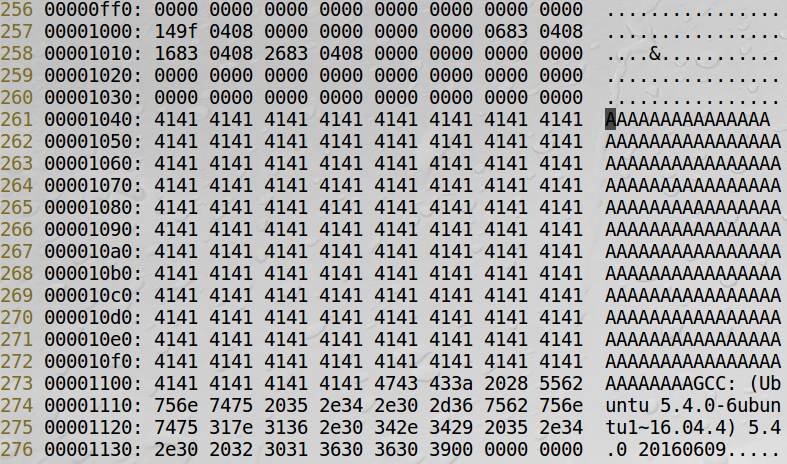
\includegraphics[scale=0.65]{pics/t3p0.png}
	\end{center}{}
	\caption{raw hex of a.out}
	\label{fig:t3p0}
\end{figure}

The first line of A' begin on line 261 (byte 4176 because 261 * 16). We want a multiple of 16 so we choose byte 4224 which is line 264. Let's retrieve all of the binary data before byte 4224 with the following command

\begin{lstlisting}[backgroundcolor = \color{lightgray},
	language = C,
	xleftmargin = 2cm,
	framexleftmargin = 1em]
$ head -c 4224 a.out > prefix
\end{lstlisting}

we then have the prefix that we can use the md5collgen program on.

\begin{lstlisting}[backgroundcolor = \color{lightgray},
language = C,
xleftmargin = 2cm,
framexleftmargin = 1em]
$ md5collgen -p prefix -o P Q
\end{lstlisting}

Finally, we need to extract the rest of the data in the program. Let's grab 128 bytes after the start of the line we chose, 4224 + 128 = 4352.

\begin{lstlisting}[backgroundcolor = \color{lightgray},
language = C,
xleftmargin = 2cm,
framexleftmargin = 1em]
$ tail -c +4352 a.out > suffix
\end{lstlisting}

Now we have all of the components to build the different executables but with the same hash!

\begin{lstlisting}[backgroundcolor = \color{lightgray},
language = C,
xleftmargin = 2cm,
framexleftmargin = 1em]
$ cat P suffix > new1
$ cat Q suffix > new2
$ md5sum new1 new2
$ chmod +x new1
$ chmod +x new2
$ echo $(./new1) | md5sum
$ echo $(./new2) | md5sum
\end{lstlisting}

The output of the previous command is shown below.

\begin{figure}[H]
	\begin{center}
		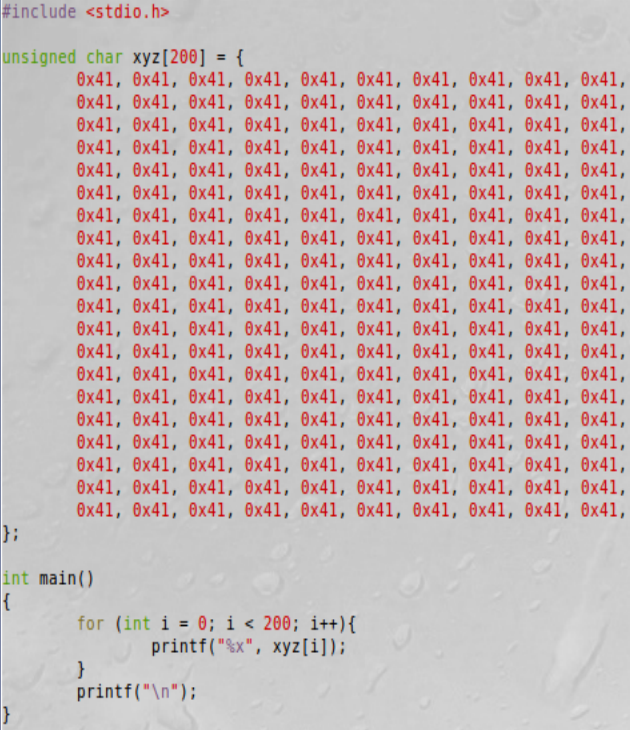
\includegraphics[scale=0.65]{pics/t3p1.png}
	\end{center}{}
	\caption{md5hash of new files}
	\label{fig:t3p1}
\end{figure}

Figure~\ref{fig:t3p1} shows the results of running md5sum on the executable files new1 and new2. These files are then executed and their output is hashes as well for simplicity in comparison. It is very easy to determine that the output of the files are different from their hash.


\subsection{Task 4: Making the Two Programs Behave Differently}
\subsubsection{Task 4: Solution}









\end{document}

